%\documentclass[mathserif]{beamer}
\documentclass[handout]{beamer}
%\usetheme{Goettingen}
\usetheme{Warsaw}
%\usetheme{Singapore}
%\usetheme{Frankfurt}
%\usetheme{Copenhagen}
%\usetheme{Szeged}
%\usetheme{Montpellier}
%\usetheme{CambridgeUS}
%\usecolortheme{}
%\setbeamercovered{transparent}
\usepackage[english, activeacute]{babel}
\usepackage[utf8]{inputenc}
\usepackage{amsmath, amssymb}
\usepackage{dsfont}
\usepackage{graphics}
\usepackage{cases}
\usepackage{graphicx}
\usepackage{pgf}
\usepackage{epsfig}
\usepackage{amssymb}
\usepackage{multirow}	
\usepackage{amstext}
\usepackage[ruled,vlined,lined]{algorithm2e}
\usepackage{amsmath}
\usepackage{epic}
\usepackage{epsfig}
\usepackage{fontenc}
\usepackage{framed,color}
\usepackage{palatino, url, multicol}
\usepackage{listings}
%\algsetup{indent=2em}


\vspace{-0.5cm}
\title{Model Evaluation and Information Criteria}
\vspace{-0.5cm}
\author[Felipe Bravo Márquez]{\footnotesize
%\author{\footnotesize  
 \textcolor[rgb]{0.00,0.00,1.00}{Felipe José Bravo Márquez}} 
\date{ \today }




\begin{document}
\begin{frame}
\titlepage


\end{frame}


%%%%%%%%%%%%%%%%%%%%%%%%%%%


\begin{frame}{Model Evaluation and Information Criteria}
\scriptsize{
\begin{itemize}
\item In this class we will introduce various concepts for evaluating statistical models.

\item According to \cite{mcelreath2020statistical}, there are two fundamental kinds of statistical error:

\begin{itemize}\scriptsize{
 \item \textbf{Overfitting}: models that learn  too much from the data leading to poor prediction.
\item \textbf{Underfitting}: models that learn too little from the data, which also leads to poor prediction.}
\end{itemize}

\item We will study the following approaches to tackle these problems.


\begin{itemize}\scriptsize{
 \item \textbf{Regularization}: a mechanism to tell our models not to get too excited by the data.
\item \textbf{Information criteria} and \textbf{Cross-validation}: scoring devices to estimate predictive accuracy of our models.}
\end{itemize}

\item In order to introduce information criteria, this class must also introduce some concepts of \textbf{information theory}.

 
\end{itemize}



} 

\end{frame}



\begin{frame}{The problem with parameters}
\scriptsize{

\begin{itemize}
\item In the class of linear regression we learned that including more attributes can lead to a more accurate model.

\item However, we also learned that adding more variables almost always improves the fit of the model to the data, as measured by the coefficient of determination $R^2$. 
\item This is true even when the variables we  add to a model have no relation to the outcome. 

\item So it's no good to choose among models using only fit to the data.






\end{itemize}


} 
\end{frame}

\begin{frame}{The problem with parameters}
\scriptsize{

\begin{itemize}

\item While more complex models fit the data better, they often predict new data worse.

\item This means that a complex model will be very sensitive to the exact sample used to fit it.

\item This will lead to potentially large mistakes when future data is not exactly like the past data.

\item But simple models, with too few parameters, tend instead to underfit, systematically over-predicting or under-predicting the data.

\item Regardless of how well future data resemble past data. 
\item So we can't always favor either simple models or complex models.

\item Let’s examine both of these issues in the context of a simple data example.

\end{itemize}


} 
\end{frame}


\begin{frame}[fragile]{The problem with parameters}
\scriptsize{

\begin{itemize}

\item We are going to create a data.frame containing  average brain volumes and body masses for seven hominin species.

\begin{verbatim}
sppnames <- c( "afarensis","africanus","habilis",
               "boisei", "rudolfensis","ergaster",
               "sapiens")
brainvolcc <- c( 438 , 452 , 612, 521, 752, 871, 
                 1350 )
masskg <- c( 37.0 , 35.5 , 34.5 , 41.5 , 55.5 , 
             61.0 , 53.5 )
d <- data.frame( species=sppnames , brain=brainvolcc,
                 mass=masskg ) 
\end{verbatim}

\item It's not unusual for data like this to be highly correlated.
\item Brain size is correlated with body size, across
species. 

\end{itemize}


} 
\end{frame}


\begin{frame}[fragile]{The problem with parameters}
\scriptsize{

\begin{figure}[h!]
	\centering
	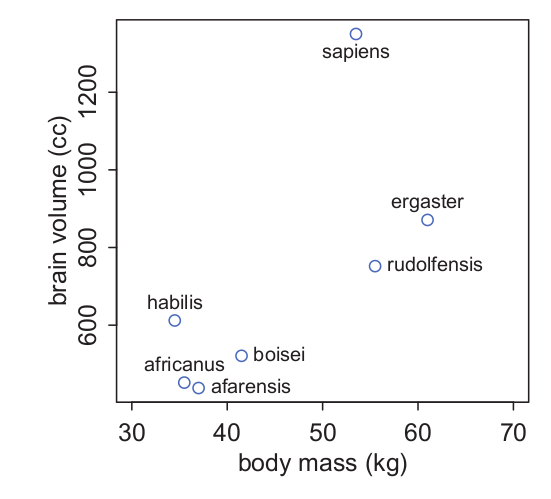
\includegraphics[scale=0.41]{pics/hominin.png}
\end{figure}


} 
\end{frame}


\begin{frame}[fragile]{The problem with parameters}
\scriptsize{

\begin{itemize}

\item We will model brain size as a function of body size.

\item We will fit a series of increasingly complex model families and see which function fits the data best.

\item Each of these models will just be a polynomial of higher degree.

\begin{verbatim}
reg.ev.1 <- lm( brain ~ mass , data=d )
reg.ev.2 <- lm( brain ~ mass + I(mass^2)
                , data=d )
reg.ev.3 <- lm( brain ~ mass + I(mass^2)
                + I(mass^3),data=d )
reg.ev.4 <- lm( brain ~ mass + I(mass^2)
                + I(mass^3) + I(mass^4),data=d )
reg.ev.5 <- lm( brain ~ mass + I(mass^2)
                + I(mass^3) + I(mass^4)
                + I(mass^5),data=d )
reg.ev.6 <- lm( brain ~ mass + I(mass^2)
                + I(mass^3) + I(mass^4)+ 
                  I(mass^5)+ I(mass^6),data=d ) 
\end{verbatim}


\end{itemize}


} 
\end{frame}

\begin{frame}[fragile]{The problem with parameters}
\scriptsize{

\begin{itemize}

\item Let's calculate $R^2$ for each of these models:

\begin{verbatim}
> summary(reg.ev.1)$r.squared
[1] 0.490158
> summary(reg.ev.2)$r.squared
[1] 0.5359967
> summary(reg.ev.3)$r.squared
[1] 0.6797736
> summary(reg.ev.4)$r.squared
[1] 0.8144339
> summary(reg.ev.5)$r.squared
[1] 0.988854
> summary(reg.ev.6)$r.squared
[1] 1
\end{verbatim}

\item As the degree of the polynomial defining the mean increases, the fit always improves.

\item The sixth-degree polynomial actually has a perfect fit, $R  ^2 = 1$.

\end{itemize}


} 
\end{frame}

\begin{frame}[fragile]{The problem with parameters}
\scriptsize{

\begin{figure}[h!]
	\centering
	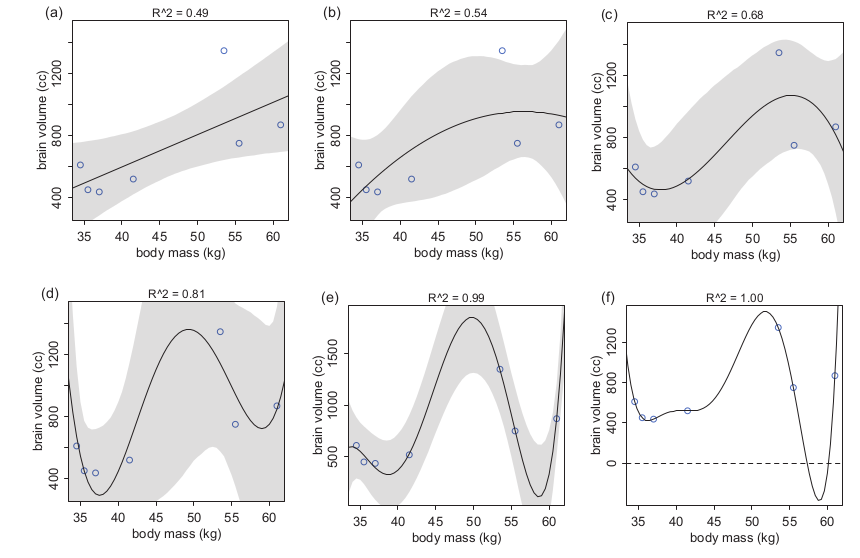
\includegraphics[scale=0.41]{pics/polyover.png}
\end{figure}

Polynomial linear models of increasing degree, fit to the hominin data. Each plot shows the predicted mean in black, with 89\% interval of the mean shaded. $R^2$, is displayed above each plot. (a) First-degree polynomial. (b) Second-degree. (c) Third-degree. (d) Fourth-degree. (e) Fifth-degree. (f) Sixth-degree. Source: \cite{mcelreath2020statistical}. 

} 
\end{frame}




\begin{frame}{The problem with parameters}
\scriptsize{

\begin{itemize}

\item We can see from looking at the paths of the predicted means that the higher-degree polynomials are increasingly absurd. 

\item For example, \textbf{reg.ev.6} the most complex model makes a perfect fit, but the model is ridiculous. 

\item Notice that there is a gap in the body mass data, because there are no fossil
hominins with body mass between 55 kg and about 60 kg. 
\item In this region, the models has nothing to predict, so it pays no price for swinging around wildly in this interval.
\item The swing is so extreme that at around 58 kg, the model predicts a negative brain size!

\item The model pays no price (yet) for this absurdity, because there are no cases in the data with body mass near 58 kg.

\end{itemize}


} 
\end{frame}



\begin{frame}{The problem with parameters}
\scriptsize{

\begin{itemize}

\item Why does the sixth-degree polynomial fit perfectly? 
\item Because it has enough parameters to assign one to each point of data.

\item The model's equation for the mean has 7 parameters:

\begin{displaymath}
 y_i=\beta_{0}+\beta_{1}x_i +\beta_{2}x_i^2 +\beta_{3}x_i^3 +\beta_{4}x_i^4 +\beta_{5}x_i^5+\beta_{6}x_i^6+\epsilon_i \quad \forall i
\end{displaymath}
and there are 7 species to predict brain sizes for.

\item So effectively, this model assigns a unique parameter to reiterate each observed brain size.
\item This is a general phenomenon: If you adopt a model family with enough parameters, you can fit the data exactly. 
\item But such a model will make rather absurd predictions for yet-to-be-observed cases.


\end{itemize}


} 
\end{frame}


\begin{frame}[fragile]{Too few parameters hurts, too}
\scriptsize{

\begin{itemize}
\item The overfit polynomial models manage to fit the data extremely well.

\item But they suffer for this within-sample accuracy by making nonsensical out-of-sample predictions.

\item In contrast, underfitting produces models that are inaccurate both
within and out of sample.

\item For example, consider this model of brain volume:

\begin{displaymath}
 y_i=\beta_{0}+\epsilon_i \quad \forall i
\end{displaymath}

\item There are no predictor variables here, just the intercept $\beta_{0}$.

\item We can fit this model as follows:

\begin{verbatim}
> reg.ev.0 <- lm( brain ~ 1 , data=d )
> summary(reg.ev.0)$r.squared
[1] 0 
\end{verbatim}

\item The value of $R^2$ is 0.

\end{itemize}


} 
\end{frame}


\begin{frame}[fragile]{Too few parameters hurts, too}
\scriptsize{

\begin{itemize}


\item This model estimates the mean brain volume, ignoring body mass.


\begin{figure}[h!]
	\centering
	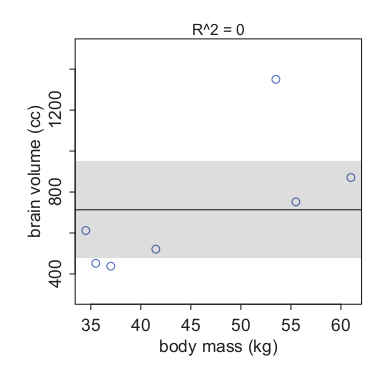
\includegraphics[scale=0.41]{pics/regconstant.png}
\end{figure}

\item As a result, the regression line is perfectly horizontal and poorly fits both smaller and larger brain volumes.

\item Such a model not only fails to describe the sample.

\item It would also do a poor job for new data.

\end{itemize}


} 
\end{frame}


\begin{frame}{Roadmap}
\scriptsize{

\begin{itemize}
\item The first thing we need to navigate between overfitting and underfitting problems is a criterion of model performance.

\item We will see how \textbf{information theory} provides a useful criterion for model evaluation: the \textbf{out-of-sample deviance}.

\item Once we learn about this criterion we will see how \textbf{cross-validation} and \textbf{information criteria} can help to estimate the out-of-sample deviance of a model.

\item We will also learn how to use \textbf{regularization} to improve the out-of-sample deviance of a model.

\item As usual, we will start with an example.

\end{itemize}


} 
\end{frame}

\begin{frame}{The Weatherperson}
\scriptsize{

\begin{itemize}
\item Suppose in a certain city, a certain weatherperson issues uncertain predictions for rain or shine on each day of the year.

\item The predictions are in the form of probabilities of rain. 

\item The currently employed weatherperson predicted these chances of rain over a 10-day sequence: 

\begin{figure}[h!]
	\centering
	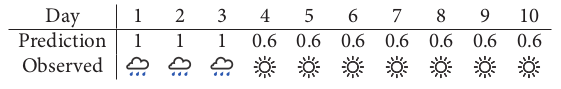
\includegraphics[scale=0.41]{pics/weather1.png}
\end{figure}


\item A newcomer rolls into town, and this newcomer boasts that he can best the current weatherperson, by always predicting sunshine. 

\item Over the same 10 day period, the newcomer's record would be:

\begin{figure}[h!]
	\centering
	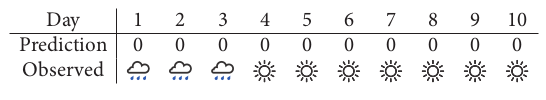
\includegraphics[scale=0.41]{pics/weather2.png}
\end{figure}


\end{itemize}


} 
\end{frame}


\begin{frame}{The Weatherperson}
\scriptsize{

\begin{itemize}
\item Define hit rate as the average chance of a correct prediction. 
\item So for the current weatherperson, she gets $3 \times 1 + 7 \times 0.4 = 5.8$ hits in 10 days, for a rate of $5.8/10 = 0.58$ correct predictions per day.
\item In contrast, the newcomer gets $3 \times 0 + 7 \times 1 = 7$, for $7/10 = 0.7$ hits per day. 
\item The newcomer wins.

\item Let's compare now the two predictions using another metric, the joint likelihood: $\prod f(y_i;\theta)$ for a frequentist model or $\prod f(y_i|\theta)$ for a Bayesian one.

\item The joint likelihood corresponds to the joint probability of correctly predicting the observed sequence.


\item To calculate it we must first compute the probability of a correct prediction for each day.

\item Then multiply all of these probabilities together to get the joint probability of correctly predicting the observed sequence. 



\end{itemize}


} 
\end{frame}

\begin{frame}{The Weatherperson}
\scriptsize{

\begin{itemize}
\item The probability for the current weather person is $1^3 \times 0.4^7 \approx 0.005$. 

\item For the newcomer, it's $0^3 \times 1^7 = 0$. 
\item So the newcomer has zero
probability of getting the sequence correct. 
\item This is because the newcomer's predictions never expect rain.
\item So even though the newcomer has a high average probability of being correct
(hit rate), he has a terrible joint probability (likelihood) of being correct.

\item And the joint likelihood is the measure we want. 

\item Because it is the unique measure that correctly counts up the relative number of ways each event (sequence of rain and shine) could happen.

\item In the statistics literature, this measure is sometimes called the
\textbf{log scoring rule}, because typically we compute the logarithm of the joint probability and report that.


\end{itemize}


} 
\end{frame}


\begin{frame}{Information and uncertainty}
\scriptsize{

\begin{itemize}
\item So we want to use the log probability of the data to
score the accuracy of competing models. 
\item The next problem is how to measure distance from
perfect prediction.
\item A perfect prediction would just report the true probabilities of rain on each day. 
\item So when either weatherperson provides a prediction that differs from the target, we can measure the distance of the prediction from the target.

\end{itemize}


} 
\end{frame}


\begin{frame}{Information and uncertainty}
\scriptsize{

\begin{itemize}

\item What kind of distance should we adopt?

\item Getting to the answer depends upon appreciating what an accuracy metric needs to do.

\item It should appreciate that some targets are just easier to hit than other targets. 
\item For example, suppose we extend the weather forecast into the winter. Now there are three types of days:
rain, sun, and snow.
\item Now there are three ways to be wrong, instead of just two.
\item This has to be reflected in any reasonable measure of distance from the target, because by adding another type of event, the target has gotten harder to hit.

\item Before presenting a distance metric that satisfies the properties described above, we must introduce some concepts from information theory.

\end{itemize}


} 
\end{frame}


\begin{frame}{Information Theory}
\scriptsize{

\begin{itemize}

\item  The field of information theory, with Claude Shannon as one of its pioneering figures, was originally applied to problems of message communication, such as the telegraph.

\begin{figure}[h!]
	\centering
	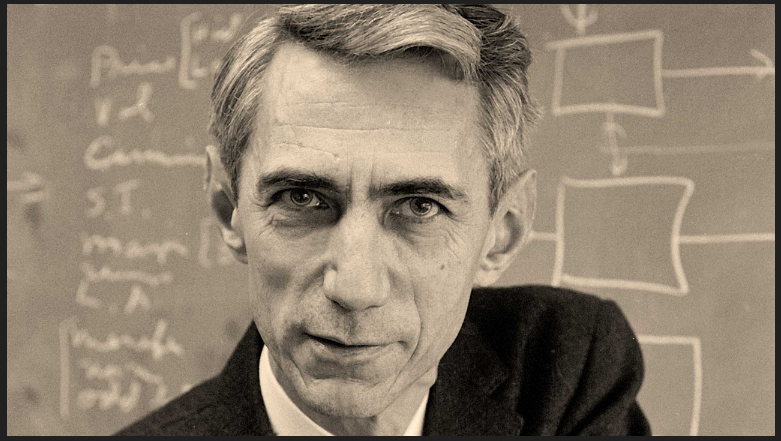
\includegraphics[scale=0.2]{pics/shannon.png}
\end{figure}
\vspace{3mm}

\item The basic insight is to ask: How can we quantify the uncertainty inherent in a probability distribution?

\end{itemize}


} 
\end{frame}


\begin{frame}{Entropy}
\scriptsize{

\begin{itemize}

\item  Information entropy is a function that measures the uncertainty on probability functions.

\item Let $X$ be a discrete random variable of $m$ different possible events, with a probaility mass function $f$, the entropy of $X$ is defnined as follows:

\begin{equation}
 H(X) = - \mathbb{E}(\log f(x)) = -\sum_{i=1}^{m}f(x_i)\log f(x_i) 
\end{equation}

\item Usually we use log base 2, in which case the entropy units are called \textbf{bits} \cite{pml1Book}.

\item If $X$ is continuous with density function $f$, the entropy $H(X)$ takes the following form:

\begin{equation}
 H(X) = - \mathbb{E}(\log f(x)) = -\int f(x)\log f(x)dx
\end{equation}

\item In plainer words: ``The uncertainty contained in a probability distribution is the negative average log-probability of an event''.


\end{itemize}


} 
\end{frame}

\begin{frame}[fragile]{Entropy}
\scriptsize{

\begin{itemize}

\item  An example will help to demystify the function $H(X)$. 

\item To compute the information entropy for the weather, suppose the true probabilities of rain ($X=1$) and shine ($X=2$) are $f(1) = \mathbb{P}(X=1)= 0.3$ and $f(2) = \mathbb{P}(X=2) = 0.7$, respectively. 

\item Then:

\begin{displaymath}
 H(X) = - (f(1)\log f(1)+\left(f(2)\log f(2)\right) \approx 0.88
\end{displaymath}

\item As an R calculation:

\begin{verbatim}
> f <- c( 0.3 , 0.7 )
> -sum( f*log2(f) )
[1] 0.8812909
\end{verbatim}


\end{itemize}


} 
\end{frame}


\begin{frame}[fragile]{Entropy}
\scriptsize{

\begin{itemize}

\item Suppose instead we live in Abu Dhabi. 

\item Then the probabilities of rain and shine might be more like $f(1) = 0.01$ and $f(2) = 0.99$. 

\begin{verbatim}
> f <- c( 0.01 , 0.99 )
> -sum( f*log2(f) )
[1] 0.08079314
\end{verbatim}


\item Now the entropy is about 0.08. 

\item Why has the uncertainty decreased? 
\item Because in Abu Dhabi it hardly ever rains. 
\item Therefore there's much less uncertainty about any given day, compared to a place in which it rains 30\% of the time.

\item These entropy values by themselves don't mean much to us, though.

\item Instead we can use them to build a measure of accuracy. That comes next.

\end{itemize}


} 
\end{frame}

\begin{frame}{Divergence}
\scriptsize{

\begin{itemize}

\item  How can we use information entropy to say how far a model is from the target? 

\item The key lies in divergence.

\item Divergence: The additional uncertainty induced by using probabilities from
one distribution to describe another distribution.

\item This is often known as \textbf{Kullback-Leibler divergence} or simply K-L divergence, named after the people who introduced it for this purpose.

\item Suppose for example that the true distribution of events is encoded by function $f$: $f(1) = 0.3$, $f(2) = 0.7$.
\item Now, suppose we believe that these events happen according to another function $q$: $q(1) = 0.25$, $q(2) = 0.75$.

\item How much additional uncertainty have we introduced, as a consequence of using $q$ to approximate $f$? 

\item  The answer is the the K-L divergence $D_{KL}(f,q)$.

\end{itemize}


} 
\end{frame}


\begin{frame}[fragile]{Divergence}
\scriptsize{

\begin{itemize}



\item If $f$ and $q$ are probability mass functions, the K-L divergence is defined as follows:

\begin{equation}
 D_{KL}(f,q) = \sum_{i=1}^m f(x_i)(\log f(x_i)-\log q(x_i)) = \sum_{i=1}^m f(x_i)\log \left(\frac{f(x_i)}{q(x_i)}\right)
\end{equation}

\begin{verbatim}
> f<-c(0.3,0.7)
> q<-c(0.25,0.75)
> sum(f* log2(f/ q)) 
[1] 0.00923535 
\end{verbatim}


\item This naturally extends to continuous density functions as well \cite{pml1Book}:

\begin{equation}
 D_{KL}(f,q) = \int f(x)\log \left(\frac{f(x)}{q(x)}\right)dx
\end{equation}


\item In plainer language, the divergence is the average difference in log probability between the target (f) and model (q). 

\item This divergence is just the difference between two entropies.

\item The entropy of the target distribution $f$ and the cross entropy arising from using $q$ to predict $f$.

\end{itemize}


} 
\end{frame}


\begin{frame}{Cross entropy and divergence}
\scriptsize{

\begin{itemize}



\item  When we use a probability distribution $q$ to predict events from another
distribution $f$, this defines something known as cross entropy $H(f,q)$:
\begin{equation}
 H(f,q) = - \sum_{i=1}^{m}f(x_i)\log q(x_i)
\end{equation}

\item The notion is that events arise according to $f$, but they are expected according to the $q$, so the entropy is inflated, depending upon how different $f$ and $q$ are.

\item Divergence is defined as the additional entropy induced by using $q$.

\item So it is the difference between $H(f)$, the actual entropy of events, and $H(f, q)$:

\begin{equation}
 D_{KL}(f,q) = H(f,q)-H(f)
\end{equation}

\item So divergence really is measuring how far q is from the target $f$, in units of entropy.

\item Notice that which is the target matters: $H(f, q)$ does not in general equal $H(q, f)$.

\end{itemize}


} 
\end{frame}


\begin{frame}[fragile]{Divergence}
\scriptsize{

\begin{itemize}

\item  When $f = q$, we know the actual probabilities of the events and the divergence becomes zero: 

 \begin{displaymath}
                     D_{KL}(f,q) =   D_{KL}(f,f) = 0
                    \end{displaymath}


\begin{verbatim}
> q <- f
> sum(f*log2(f/ q)) 
[1] 0
\end{verbatim}
                    
\item As q grows more different from $f$, the divergence $D_{KL}$ also grows.       
       
\item Suppose the true target distribution is $f = \{0.3, 0.7\}$.

\item Suppose the approximating distribution q can be anything from $q = \{0.01, 0.99\}$ to $q = \{0.99, 0.01\}$.       
       
\item Let's build a plot with $q(1)$ on the horizontal axis and the divergence $D_{KL}(f, q)$ on vertical one.       
       
\end{itemize}


} 
\end{frame}

\begin{frame}[fragile]{Divergence}
\scriptsize{

\begin{verbatim}
t <- 
  tibble(f_1  = .3,
         f_2  = .7,
         q_1  = seq(from = .01, to = .99, by = .01)) %>% 
  mutate(q_2  = 1 - q_1) %>%
  mutate(d_kl = (f_1 * log2(f_1 / q_1)) + (f_2 * log2(f_2 / q_2)))

t %>% 
  ggplot(aes(x = q_1, y = d_kl)) +
  geom_vline(xintercept = .3,  linetype = 2) +
  geom_line(size = 1.5) +
  annotate(geom = "text", x = .4, y = 1.5, label = "q = f", 
           size = 3.5) +
  labs(x = "q(1)",
       y = "Divergence of q from f") 
\end{verbatim}



} 
\end{frame}

\begin{frame}{Divergence}
\scriptsize{

\begin{figure}[h!]
	\centering
	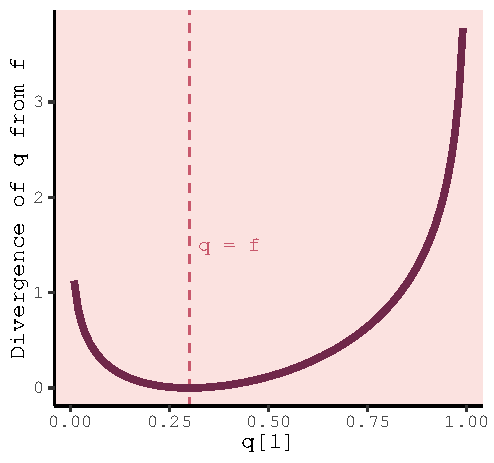
\includegraphics[scale=0.45]{pics/divergence.pdf}
\end{figure}

\begin{itemize}
 \item Only exactly where $q = f$, at $q(1) = 0.3$, does the divergence achieve a value of zero. Everyplace else, it grows.
 
 \item Since predictive models specify probabilities of events (observations), we can use divergence to compare the accuracy of models. 
\end{itemize}


} 
\end{frame}


\begin{frame}{Estimating divergence}
\scriptsize{

\begin{itemize}

\item  To use $D_{KL}$ to compare models, it seems like we would have to know $f$, the target probability distribution.
\item In all of the examples so far, I've just assumed that $f$ is known.
\item But when we want to find a model $q$ that is the best approximation to $f$, the ``truth,'' there is usually no way to access $f$ directly.
\item We wouldn't be doing statistical inference, if we already knew $f$.

\item But there's an amazing way out of this predicament. 
\item It helps that we are only interested in comparing the divergences of different candidates, say $q$ and $r$. 
\item In that case, most of $f$ just subtracts out, because there is a $\mathbb{E}(\log f(x))$ term in the divergence of both q and r.
\item This term has no effect on the distance of q and r from one another. 

\end{itemize}


} 
\end{frame}


\begin{frame}{Estimating divergence}
\scriptsize{

\begin{itemize}

\item So while we don't know where $f$ is, we can estimate how far apart $q$ and $r$ are, and which is closer to the target.


\item All we need to know is a model's average log-probability: $\mathbb{E}(\log q(x))$ for q and $\mathbb{E}(\log r(x))$ for r. 



\item To approximate the relative value of $\mathbb{E}(\log q(x))$, we can use the log-probability score of the model:

\begin{equation}
S(q) = \sum_{i=1}^m \log q(x_i)
\end{equation}


\item This sore is an estimate of $\mathbb{E}(\log q(x))$, just without the final step of dividing by the number of observations.

\item It is also an approximation of the K-L divergence of the model relative to the unknown target model. 


\end{itemize}


} 
\end{frame}

\begin{frame}[fragile]{Calculating Log-Likelihood}
\scriptsize{

\begin{itemize}




\item Most of the standard model fitting functions in R support ``logLik'' , which computes the sum of log-probabilities, usually known as the log-likelihood of the data.

\begin{verbatim}
> logLik(reg.ev.1)
'log Lik.' -47.46249 (df=3)
> logLik(reg.ev.2)
'log Lik.' -47.13276 (df=4) 
\end{verbatim}

\item Recall that the absolute magnitude of these values are not interpretable.

\item Only the difference  $S(q) - S(r)$ informs us about the divergence of each model from the unknown target $f$.

\item We can calculate the log-likelihood of a model by hand using the following code:

\begin{verbatim}
b0<-reg.ev.1$coefficients[1]
b1<-reg.ev.1$coefficients[2]

logLik1 <- sum(log(dnorm(
  d$brain ,
  mean=b0+b1*d$mass ,
  sd=sigma(reg.ev.1))
  ))
> logLik1
[1] -47.64015
\end{verbatim}


\end{itemize}


} 
\end{frame}

\begin{frame}[fragile]{Calculating Log-Likelihood}
\scriptsize{

\begin{itemize}




\item Note that this log-likelihood differs from the one obtained with \verb+logLik+.

\item This is because \verb+sigma(reg.ev.1)+ returns an unbiased estimator of $\sigma$: \begin{displaymath}
   \hat{\sigma} = \sqrt{\frac{\sum \epsilon_i^2}{df}}
                                                                                        \end{displaymath}
where $df=n-2=7-2=5$.

\begin{verbatim}
> sigma(reg.ev.1)
[1] 252.0567
> reg.ev.1$df.residual
[1] 5
> sigma.LM <-sqrt(sum(reg.ev.1$residuals^2)/
+                   reg.ev.1$df.residual)
> sigma.LM
[1] 252.0567
\end{verbatim}



\end{itemize}


}
\end{frame}


\begin{frame}[fragile]{Calculating Log-Likelihood}
\scriptsize{

\begin{itemize}

\item On the other hand, the function \verb+logLik+ uses the maximum likelihood estimator of $\sigma$:
\begin{displaymath}
 \hat{\sigma}_{ML} = \sqrt{\frac{\sum \epsilon_i^2}{n}}
\end{displaymath}

\begin{verbatim}
sigma.ML<-sqrt(sum(reg.ev.1$residuals^2)
               /dim(d)[1])

> sigma.ML
[1] 213.0268

logLik1.1 <- sum(log(dnorm(
  d$brain ,
  mean=b0+b1*d$mass ,
  sd=sigma.ML)
))
> logLik1.1
[1] -47.46249
\end{verbatim}



\end{itemize}


}
\end{frame}


\begin{frame}[fragile]{Calculating Log-Likelihood}
\scriptsize{

\begin{itemize}

\item We can obtain the same results using MAP estimates from a Bayesian model with flat priors:

\begin{verbatim}
library(rethinking)
b.reg.ev.1<- quap(
  alist(
    brain ~ dnorm( mu , sigma ) ,
    mu <- b0 + b1*mass
  ) ,
  data=d ,
  start=list(b0=mean(d$brain),b1=0,sigma=sd(d$brain)) ,
  method="Nelder-Mead" )

theta <- coef(b.reg.ev.1)
logLik1.2 <- sum(log(dnorm(
  d$brain ,
  mean=theta[1]+theta[2]*d$mass ,
  sd=theta[3])
  ))

> logLik1.2
[1] -47.46249
\end{verbatim}



\end{itemize}


}
\end{frame}


\begin{frame}[fragile]{Deviance}
\scriptsize{

\begin{itemize}

\item It is also quite common to see something called the \textbf{deviance}, which is $S(q)$ multiplied by -2.

\begin{equation}
D(q) = -2\times S(q)= -2 \sum_{i=1}^n \log q(x_i)
\end{equation}


\item The 2 is there for historical reasons.

\item When comparing the deviance,  smaller values are better.  

\begin{verbatim}
> -2*logLik(reg.ev.1)
'log Lik.' 94.92499 (df=3)
> -2*logLik(reg.ev.2)
'log Lik.' 94.26553 (df=4)
> -2*logLik(reg.ev.3)
'log Lik.' 91.66948 (df=5)
> -2*logLik(reg.ev.4)
'log Lik.' 87.85016 (df=6) 
\end{verbatim}



\end{itemize}


} 
\end{frame}


\begin{frame}{From deviance to out-of-sample}
\scriptsize{

\begin{itemize}

\item Deviance has the same flaw as $R^2$: It always improves as the model gets more complex.

\item It is really the deviance on new data that interests us.

\item When we usually have data and use it to fit a statistical model, the data comprise a \textbf{training sample}.

\item Parameters are estimated from it.

\item Then we can imagine using those estimates to predict outcomes in a new sample, called the \textbf{test sample}.

\item We can compute the deviance on the test sample to obtain the \textbf{out-of-sample deviance}. 

\item Let's explore it with an example.

\end{itemize}


} 
\end{frame}


\begin{frame}{From deviance to out-of-sample}
\scriptsize{

\begin{itemize}

\item Suppose we have the following data generation process and we fit linear regressions with between 1 and 5 free parameters to the data:

\begin{figure}[h!]
	\centering
	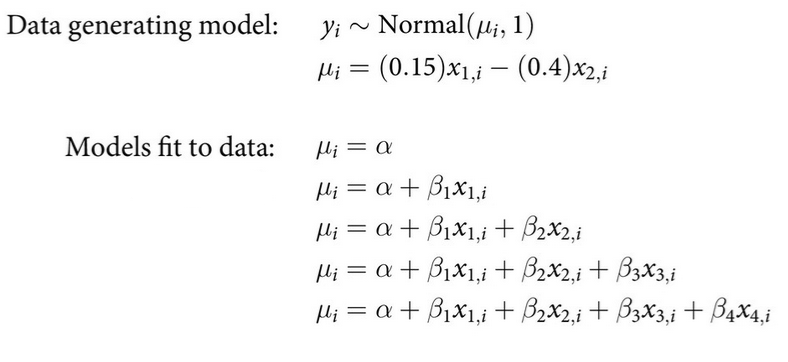
\includegraphics[scale=0.4]{pics/dev_ex.png}
\end{figure}


\item Since the ``true'' model has non-zero coefficients for only the first two predictors, we can say that the true model has 3 parameters.

\item In other words, $x_{3}$ and $x_{4}$ as uncorrelated with $y$.

\end{itemize}


} 
\end{frame}

\begin{frame}{From deviance to out-of-sample}
\scriptsize{

\begin{itemize}

\item The following diagram shows in-sample and out-of-sample deviance scores for $10,000$ simulations of 20 training and 20 testing data points from our data generation process.
\end{itemize}


\begin{figure}[h!]
	\centering
	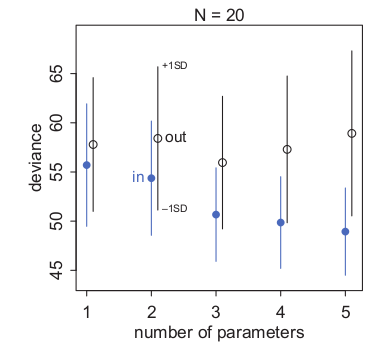
\includegraphics[scale=0.5]{pics/dev_ex2.png}
\end{figure}






} 
\end{frame}


\begin{frame}{From deviance to out-of-sample}
\scriptsize{

\begin{itemize}



\item Models with different numbers of predictor variables are shown on the horizontal axis.

\item Deviance across 10,000 simulations is shown on the vertical. 

\item Blue shows deviance in-sample, the training data. 
\item Black shows deviance out-of-sample, the test data. 
\item Points show means, and the line segments show $\pm$ 1 standard
deviation.

\item A smaller deviance means a better fit. 


\end{itemize}


} 
\end{frame}


\begin{frame}{From deviance to out-of-sample}
\scriptsize{

\begin{itemize}


\item Regarding the in-sample deviance we see that with increasing numbers of parameters, the average deviance declines. 
\item This is the same phenomenon we saw earlier with $R^2$.

\item On the other hand, the out-of-sample deviance is smallest on average for 3 parameters, which is the data-generating model
\item And it gets worse (increases) with the addition of each parameter after the third.

\item The point of this thought experiment is to demonstrate how deviance behaves, in theory. 
\item While deviance on training data always improves with additional predictor variables, deviance on future data may or may not.



\end{itemize}


} 
\end{frame}



\begin{frame}{Cross Validation}
\scriptsize{

\begin{itemize}
\item We just showed how to estimate the out-of-sample deviance by  evaluating the model on observations that were not used to fit the model. 

\item However, in many cases, we do not want to waste a portion of our data just for evaluation. 

\item So what is usually done is \textbf{cross-validation}: to divide the sample in a number of chunks, called ``folds''. 
\item Then the model is asked to predict each fold, after training on all the others.
\item We then average over the score (e.g., deviance) for each fold to get an estimate of out-of-sample performance. 
\item The minimum number of folds is 2. 
\item At the other extreme, you could make each point observation a fold and fit as many models as you have individual observations.
\item This is called leave-one-out cross-validation (often abbreviated as LOOCV).
\item The key trouble with leave-one-out cross-validation is that, if we have 1000 observations, that means computing 1000 models.
\item That can be time consuming.
\end{itemize}


} 
\end{frame}


\begin{frame}{Cross Validation}
\scriptsize{

\begin{figure}[h!]
	\centering
	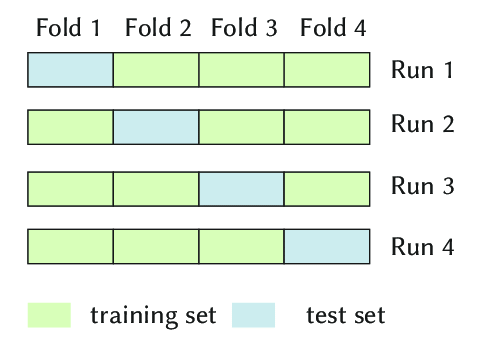
\includegraphics[scale=0.4]{pics/crossvalidation.png}
\end{figure}

} 
\end{frame}




\begin{frame}{Regularization}
\scriptsize{

\begin{itemize}

\item The root of overfitting is a model's tendency to get overexcited by the training sample.

\item One way to prevent a linear model to overfit the training data is regularization.

\item  From a frequentist point of view, the most popular regularization technique is \textbf{ridge regression}.


\item In this approach we penalize large parameter values $\beta$ in the likelihood function.

\item We add a penalization term to the target function SSE to keep  the squares of the parameter values low:

\begin{equation}
 \operatorname{argmin}_{\beta} SSE(\beta) + \lambda \sum_{j=0}^m\beta_j^2 
\end{equation} 

\item The value of $\lambda$ is an hyper-parameter that controls the ammount of overfitting.



\end{itemize}


} 
\end{frame}


\begin{frame}[fragile]{Regularization}
\scriptsize{

\begin{itemize}

\item If $\lambda$ is zero, we are just doing least mean squares.

\item If it is too large, on the other hand, we risk underfitting.

\item This value is usually ``tuned'' on an independent partition of data referred to as ``validation set''. 

\item The function lm.ridge built into R's MASS library implements the ridge regression method. 

\begin{verbatim}
library(MASS)
rid.ev.4<- lm.ridge(brain ~ mass + I(mass^2)
         + I(mass^3) + I(mass^4),data=d,lambda = 0.1) 

> rid.ev.4
                       mass     I(mass^2) 
 6.725187e+01  9.751407e+00  7.235780e-02 
    I(mass^3)     I(mass^4) 
 4.874209e-04 -1.289110e-06         
\end{verbatim}



\end{itemize}


} 
\end{frame}

\begin{frame}{Regularization}
\scriptsize{

\begin{itemize}

\item Ridge regression is an example of how a statistical procedure can be understood from both Bayesian and non-Bayesian perspectives.

\item From a Bayesian point of view, ridge regression is equivalent to setting a Gaussian prior centered at zero for each $\beta$ coefficient.

\item In this setting, the value of $\sigma$ controls the ammount of regularization.

\item For example, a prior $\beta \sim $Normal$(0, 1)$ says that, before seeing the data, the machine should be very skeptical of values above 2 and below -2.

\item In the next slide, we repeat the experiment of computing  the in-sample and out-of-sample deviance for models with different number of attributes using different regularization priors.

\item The data generation process is the same as before.

\end{itemize}


} 
\end{frame}


\begin{frame}{Regularization}
\scriptsize{

\begin{figure}[h!]
	\centering
	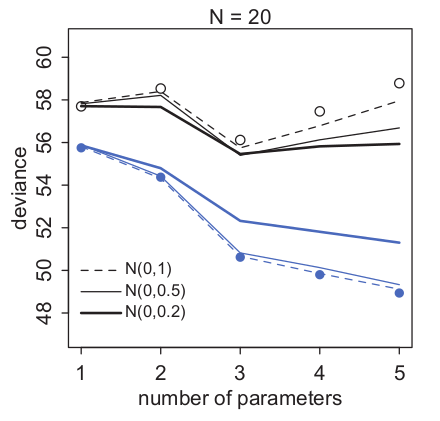
\includegraphics[scale=0.4]{pics/regularization.png}
\end{figure}

\begin{itemize}

\item The points in both plots are the same as in previous figure (no regularization).

\item The lines show training (blue) and testing (black) deviance for three regularizing priors.

\item Dashed: Each beta-coefficient is given a Normal(0, 1) prior. Thin solid: Normal(0, 0.5). Thick solid: Normal(0, 0.2).

\end{itemize}


} 
\end{frame}


\begin{frame}{Regularization}
\scriptsize{


\begin{itemize}

\item The training deviance always increases (gets worse) with tighter priors. 
\item The thick blue trend is substantially larger than the others.

\item This is because the skeptical prior prevents the model from adapting completely to the sample. 
\item But the test deviances, out-of-sample, improve (get smaller) with the tighter priors. 
\item The model with three parameters is still the best model out-of-sample.
\item The regularizing priors have little impact on its deviance.

\item But also notice that as the prior gets more skeptical, the harm done by an overly complex model is greatly reduced.
\item For the Normal(0, 0.2) prior (thick line), the models with 4 and 5 parameters are barely worse than the correct model with 3 parameters. 
\item If we can tune the
regularizing prior right, then overfitting can be greatly reduced.


\end{itemize}


} 
\end{frame}


\begin{frame}{Information criteria}
\scriptsize{

\begin{itemize}
\item Information criteria are a group of scoring devices that construct a theoretical estimate of the relative out-of-sample deviance using just the training data.
\item They are a cheaper alternative to cross-validation.

\item The most known information criterion is the \textbf{Akaike information criterion}, abbreviated AIC. 
\item AIC provides a surprisingly simple estimate of the average out-of-sample deviance:
\begin{equation}
AIC = D_{\text{train}} + 2p 
\end{equation}


where  $D_{\text{train}}$ is the in-sample deviance, and $p$ is the number of free parameters to be estimated in the model.

\item In a linear regression model, $p$ equals to the number of $\beta$ coefficients (including the intercept)  plus 1, to account to the model's standard deviation $\sigma$.


\end{itemize}


} 
\end{frame}


\begin{frame}[fragile]{Akaike information criterion}
\scriptsize{

\begin{itemize}
\item We can calculate AIC for the ``reg.ev.1'' model as follows:

\begin{verbatim}
> -2*logLik(reg.ev.1)+2*3
'log Lik.' 100.925 (df=3) 
\end{verbatim}

\item In this model $p=3$, two $\beta$ coefficients ($\beta_0,\beta_1$) and $\sigma$.

\item AIC can be computed directly in R using the ``AIC'' function:

\begin{verbatim}
> AIC(reg.ev.1)
[1] 100.925
> AIC(reg.ev.2)
[1] 102.2655
> AIC(reg.ev.3)
[1] 101.6695
> AIC(reg.ev.4)
[1] 99.85016
> AIC(reg.ev.5)
[1] 82.16384 
\end{verbatim}

\item In AIC, the lower the better, so the criterion is still preferring overfitted models in this example.


\end{itemize}


} 
\end{frame}

\begin{frame}{Akaike information criterion}
\scriptsize{

\begin{itemize}
\item Let's try to understand with an example where the AIC formula comes from.\footnote{A more detailed derivation can be found here: \url{https://barumpark.com/blog/2018/aic-and-bic/}}

\item The figure below shows again the in-sample and out-of-sample deviances for the simulated data.

\begin{figure}[h!]
	\centering
	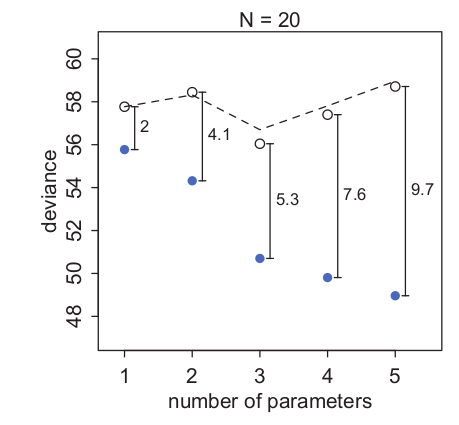
\includegraphics[scale=0.33]{pics/akaike.png}
\end{figure}


\end{itemize}


} 
\end{frame}

\begin{frame}{Akaike information criterion}
\scriptsize{

\begin{itemize}

\item The vertical line segments measure the average distance between training deviance (blue) and test
deviance (open black).

\item Each distance is nearly twice the number of parameters, as labeled on the horizontal axis. 

\item The dashed lines show exactly the blue points plus
twice the number of parameters, tracing closely along the average out-of-sample deviance for each model.

\item These lines therefore show AIC for each model, an approximation of the out-of-sample deviance.


\end{itemize}


} 
\end{frame}


\begin{frame}{Information criteria}
\scriptsize{

\begin{itemize}
\item AIC provides an approximation of predictive accuracy, as measured by out-of-sample deviance. 

\item All information criteria aim at this same target, but are derived under more and less general assumptions.

\item AIC is just the oldest and most restrictive.
\item AIC is commonly used in frequentist models fitted with maximum likelihood estimation.

\item When employed in a Bayesian setting, it assumes that the priors are flat and the posterior is approximately a multivariate Gaussian.

\item Two more-general criteria are the  Deviance Information Criterion (DIC) and the Widely Applicable Information Criterion (WAIC). 

\item DIC accommodates informative priors, but still assumes that the posterior is multivariate
Gaussian. 
\item WAIC is more general yet, making no assumption about the shape of the posterior.
\item We will only study DIC in this class.

\end{itemize}


} 
\end{frame}


\begin{frame}{Deviance Information Criterion (DIC)}
\scriptsize{

\begin{itemize}

\item The Deviance Information Criterion (DIC) is a widely used and easy to compute Bayesian information criterion. 
\item  DIC is essentially a version of AIC that is aware of informative priors.
\item Like AIC, it assumes a multivariate Gaussian posterior distribution. 
\item This means if any parameter in the posterior is substantially skewed, and also has a substantial effect on prediction, then DIC like AIC can go horribly wrong.

\end{itemize}


} 
\end{frame}


\begin{frame}{Deviance Information Criterion (DIC)}
\scriptsize{

\begin{itemize}
\item DIC is calculated from the posterior distribution of the training deviance.
\item What does it mean for the deviance to have a posterior distribution?
\item Since the parameters have a posterior distribution, and since the deviance is computed from the parameters, deviance must also have a posterior distribution.  
\item Classical ``deviance'' is defined at the
MAP values.
\item But in principle the posterior distribution provides information about predictive uncertainty.
\item That uncertainty turns out to help us estimate out-of-sample deviance.


\end{itemize}


} 
\end{frame}


\begin{frame}{Deviance Information Criterion (DIC)}
\scriptsize{

\begin{itemize}
\item So define $D$ now as the posterior distribution of deviance. 
\item This means we compute deviance (on the training sample) for each set of sampled parameter values in the posterior distribution. 
\item So if we draw $10,000$ samples from the posterior, we compute 10,000 deviance values. 
\item Let $\overline{D}$ indicate the average of $D$. 
\item Also define $\hat{D}$ as the deviance calculated at the posterior mean. 
\item This means we compute the average of each parameter in the posterior distribution. 
\item Then we plug those averages into the deviance formula to get $\hat{D}$ out.
\item Once you have $\overline{D}$ and $\hat{D}$, DIC is calculated as:

\begin{equation}
DIC = \overline{D}+ (\overline{D}-\hat{D}) =  \overline{D} + p_D
\end{equation}



\end{itemize}


} 
\end{frame}


\begin{frame}{Deviance Information Criterion (DIC)}
\scriptsize{

\begin{itemize}
\item The difference $\overline{D}-\hat{D} = p_D$ is analogous to the number of parameters used in computing AIC.
\item It is an ``effective'' number of parameters that measures how flexible the model is in
fitting the training sample. 
\item More flexible models entail greater risk of overfitting. 
\item So this $p_D$ term is sometimes called a penalty term.
\item It is just the expected distance between the deviance  in-sample and the deviance out-of-sample.
\item In the case of flat priors, DIC reduces directly to AIC, because the expected distance is just the number of parameters. 
\item But more generally, $p_D$  will be some fraction of the number of parameters, because regularizing priors constrain a model's flexibility.
\item The function ``DIC'' in the ``rethinking'' package will compute DIC for a model fit with ``quap'' or ``ulam''.

\end{itemize}


} 
\end{frame}


\begin{frame}[fragile]{Deviance Information Criterion (DIC)}
\scriptsize{

\begin{itemize}
\item Let's compare DIC for three Bayesian linear models for the Howell data.

\item b.reg1: a simple linear regression of height using weight as a predictor.

\item b.reg2: a multivariate linear regression of height using weight and age as predictors.

\item b.reg3: a polynomial regression of height using weight and weight square as predictors.

\begin{verbatim}
library(rethinking)
data(Howell1)
d <- Howell1
d2 <- d[ d$age >= 18 , ]

b.reg1 <- quap(
  alist(
    height ~ dnorm( mu, sigma ),
    mu <- b0 + b1*weight,
    b0 ~ dnorm( 150 , 50 ) ,
    b1 ~ dnorm( 0 , 1) ,
    sigma ~ dunif( 0 , 50 )
  ) , data=d2 )

\end{verbatim}



\end{itemize}


} 
\end{frame}


\begin{frame}[fragile]{Deviance Information Criterion (DIC)}
\scriptsize{

\begin{verbatim}
b.reg2 <- quap(
  alist(
    height ~ dnorm( mu, sigma ),
    mu <- b0 + b1*weight+b2*age,
    b0 ~ dnorm( 150 , 50 ) ,
    b1 ~ dnorm( 0 , 1) ,
    b2 ~ dnorm( 0 , 1) ,
    sigma ~ dunif( 0 , 50 )
  ) , data=d2 )

b.reg3 <- quap(
  alist(
    height ~ dnorm( mu, sigma ),
    mu <- b0 + b1*weight+b2*weight^2,
    b0 ~ dnorm( 150 , 50 ) ,
    b1 ~ dnorm( 0 , 1) ,
    b2 ~ dnorm( 0 , 1) ,
    sigma ~ dunif( 0 , 50 )
  ) , data=d2 )
\end{verbatim}






} 
\end{frame}


\begin{frame}[fragile]{Deviance Information Criterion (DIC)}
\scriptsize{


\begin{itemize}
\item Let's compute DIC for each model: 

\begin{verbatim}
> DIC(b.reg1)
[1] 2148.409
attr(,"pD")
[1] 3.190277
> DIC(b.reg2)
[1] 2149.218
attr(,"pD")
[1] 3.941273
> DIC(b.reg3)
[1] 2149.858
attr(,"pD")
[1] 3.805133
\end{verbatim}


\item In this case the lowest (better) score in achieved by the simplest model.

\item What we have just done is to use the DIC information criterion for model comparison.


\end{itemize}


} 
\end{frame}


\begin{frame}{Deviance Information Criterion (DIC)}
\scriptsize{


\begin{itemize}
\item With the definition of DIC in hand, let's review one more simulation exercise.

\begin{figure}[h!]
	\centering
	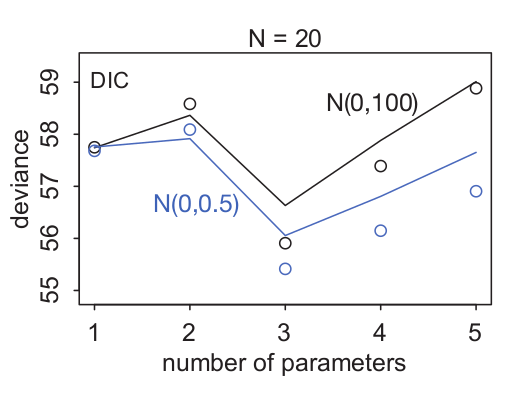
\includegraphics[scale=0.5]{pics/DIC.png}
\end{figure}

\item The figure above shows the results of 10,000 simulations each for the five familiar models with
between 1 and 5 parameters. 



\end{itemize}


} 
\end{frame}


\begin{frame}{Deviance Information Criterion (DIC)}
\scriptsize{


\begin{itemize}
 
\item The plot displays only out-of-sample deviance now, for simplicity. 
\item The black points are average out-of-sample deviance resulting from simulations with nearly flat priors.
\item The blue points result from simulations using regularizing Normal(0, 0.5)
priors. 
\item The black and blue lines show the estimated out-of-sample deviance from DIC, with colors corresponding to groups of points.

\item DIC is an accurate estimate of out-of-sample deviance, being within 1 point of deviance of the actual average in most cases.




\end{itemize}


} 
\end{frame}


\begin{frame}{Deviance Information Criterion (DIC)}
\scriptsize{


\begin{itemize}
 


\item Also notice that the regularizing prior (blue) still helps, and that DIC tracks this help.
\item This suggests that using both regularization and information criteria will always beat using only one or the other alone. 
\item Regularization, as long as it's not too strong, reduces  overfitting for any particular model. \item Information criteria instead help us measure overfitting across models fit to the same data. 
\item These are complementary functions. 
\item And since both are very easy to use and widely available, there's no reason to shy away from their use.


\end{itemize}


} 
\end{frame}


\begin{frame}{Conclusions}
\scriptsize{

\begin{itemize}
\item This class has been a marathon. 
\item It began with the problem of overfitting, a universal phenomenon by which models with more parameters fit a sample better, even when the additional parameters are meaningless.
\item Theree common tools were introduced to address over-fitting: regularization, cross-validation, and information criteria.
\item Regularization reduces overfitting during estimation, and both cross-validation and information criteria help estimate the degree of overfitting. 
\item In all cases, keep in mind that these tools are heuristic. 
\item They provide no guarantees. 
\item No statistical procedure will ever substitute for iterative scientific investigation.
\end{itemize}


} 
\end{frame}


%%%%%%%%%%%%%%%%%%%%%%%%%%%
\begin{frame}[allowframebreaks]\scriptsize
\frametitle{References}
\bibliography{bio}
\bibliographystyle{apalike}
%\bibliographystyle{flexbib}
\end{frame}  









%%%%%%%%%%%%%%%%%%%%%%%%%%%

\end{document}
